% preamble ---------------------------------------------------------------
\documentclass[xcolor=dvipsnames]{beamer}

% meta data --------------------------------------------------------------
\title[Text supporting CV models]{Seminar: Multimodal Deep Learning}
\subtitle{Topic 7: Text supporting CV models}
\author[Max Schneider]{Author: Maximilian Schneider\\
        Supervisor: Jann Goschenhofer}
\institute[]{Department Of Statistics\\
             Ludwig-Maximilians-Universität\\
             \vspace{0.5cm}
             
\includegraphics[scale=0.02]{figures/Sigillum}%
            }
\date{\today}

% theme
\usetheme{Madrid}
\usecolortheme{dove}
\beamertemplatenavigationsymbolsempty  % no navigations symbols
\setbeamertemplate{section in toc}{\hspace*{1em}\textcolor{OliveGreen}{\inserttocsectionnumber}~\inserttocsection\par}
\setbeamertemplate{subsection in toc}{\hspace*{2em}\textcolor{OliveGreen}{\inserttocsectionnumber.\inserttocsubsectionnumber}~\inserttocsubsection\par}  % numbered table of contents
\setbeamercovered{transparent}
\usefonttheme[onlymath]{serif}  % better math font
\setbeamertemplate{caption}[numbered]

% packages ---------------------------------------------------------------
% text encoding
\usepackage[utf8]{inputenc}

% better interaction with pdf (strg + f)
\usepackage[T1]{fontenc}

% comment, quote environment (load csquotes before babel)
\usepackage{comment, csquotes}

% language, line breaks
\usepackage[english]{babel}

% date format
\usepackage[datesep=.]{datetime2}
\DTMsetdatestyle{ddmmyyyy}

% bibliography
\usepackage[style=authoryear, backend=biber, sorting=nty, uniquename=false]{biblatex}
\addbibresource{../../book.bib}
% \addbibresource{sources.bib}
\renewcommand*{\bibsetup}{%
  \interlinepenalty=10000\relax % default is 5000
  \widowpenalty=10000\relax
  \clubpenalty=10000\relax
  \raggedbottom
  \frenchspacing
  \biburlsetup}

% load external figures, embed functioning links
\usepackage{graphicx, hyperref}

% sub-figures
\usepackage{caption, subcaption}

% one table cell over multiple columns
\usepackage{multicol}

% math symbols
\usepackage{amsmath, amssymb, bm}

\begin{document} %--------------------------------------------------------

{
\setbeamertemplate{footline}{}
\begin{frame}
  \titlepage
\end{frame}
}
\addtocounter{framenumber}{-1}

\section{Introduction} %--------------------------------------------------

\begin{frame}{Introduction: Scale}
  \blockquote{
    The biggest lesson that can be read from 70 years of AI research is that general methods that leverage computation are ultimately the most effective, and by a large margin.
    \ldots
    Most AI research has been conducted as if the computation available to the agent were constant (in which case leveraging human knowledge would be one of the only ways to improve performance) but, over a slightly longer time than a typical research project, massively more computation inevitably becomes available.
    Seeking an improvement that makes a difference in the shorter term, researchers seek to leverage their human knowledge of the domain, but the only thing that matters in the long run is the leveraging of computation.
    \ldots
  }
\end{frame}

\begin{frame}{Introduction: Scale}
  \blockquote[\cite{sutton2019bitterlesson}]{
    \ldots
    One thing that should be learned from the bitter lesson is the great power of general purpose methods, of methods that continue to scale with increased computation even as the available computation becomes very great.
    The two methods that seem to scale arbitrarily in this way are search and learning.
  }
\end{frame}

\section{Concepts} %------------------------------------------------------
\begin{frame}{Contents}
  \tableofcontents[sections={1-2}, currentsection]
  \tableofcontents[sections={3-6}]
\end{frame}

\subsection{Web-scale data} %---------------------------------------------
\begin{frame}{Concepts: Web-scale data}
  \begin{itemize}
    \item Possible through natural language supervision
    \item No labor intensive manual labeling
    \item Large datasets
      \begin{itemize}
        \item 400 million \parencite[CLIP;][]{radford2021learning}
        \item 900 million \parencite[Florence;][]{yuan2021florence}
        \item 1.8 billion \parencite[ALIGN;][]{jia2021scaling}
      \end{itemize}
    \item Pre-processing needed, resulting in arbitrary choices
    \item Social biases are reproduced
  \end{itemize}
\end{frame}

\subsection{Contrastive objective} %--------------------------------------
\begin{frame}{Concepts: Contrastive objective}
  \begin{equation}
    \ell^{V1, V2} = - \underset{\{v_1^1, v_2^1, \ldots, v_2^{k+1}\}}{\mathbb{E}} \left( \log \frac{h_\theta(\{v_1^1,v_2^1\})}{h_\theta(\{v_1^1,v_2^1\}) + \sum_{j=2}^{k+1} h_\theta(\{v_1^1, v_2^j\})} \right)
  \end{equation}

  \vspace{1cm}

  \begin{figure}[ht]
    \begin{minipage}{0.67\textwidth}
      \centering
      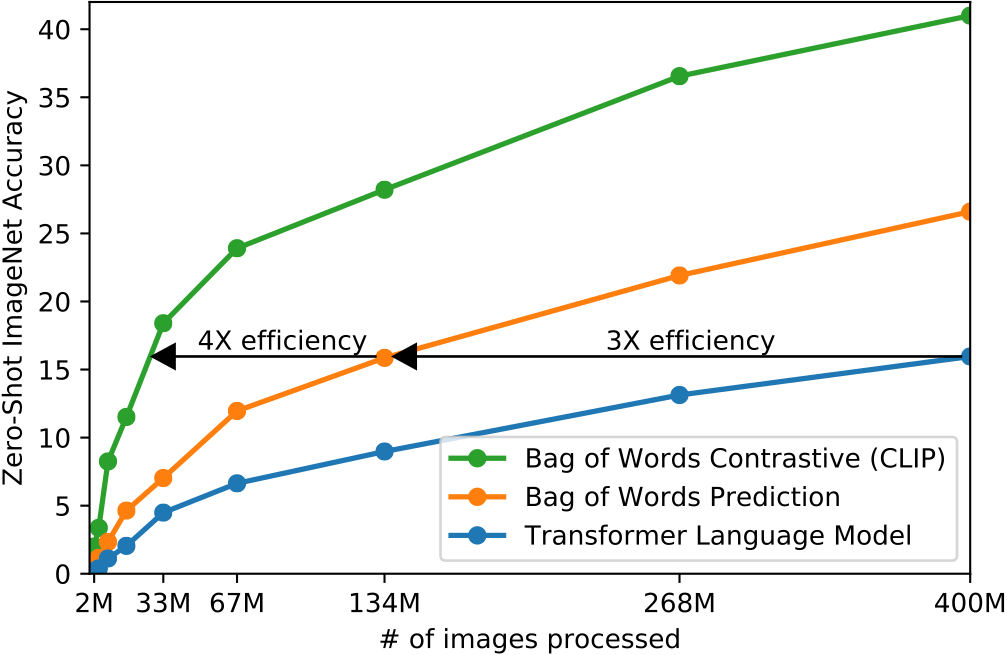
\includegraphics[width=0.9\linewidth]{../../figures/02-04-text-support-img/data-efficiency}
    \end{minipage}
    \begin{minipage}[c]{0.3\textwidth}
      \caption{Data efficiency of contrastive objective \parencite{radford2021learning}}
    \end{minipage}
  \end{figure}
\end{frame}

\begin{frame}{Concepts: Contrastive objective}
  \begin{figure}[ht]
    \centering
    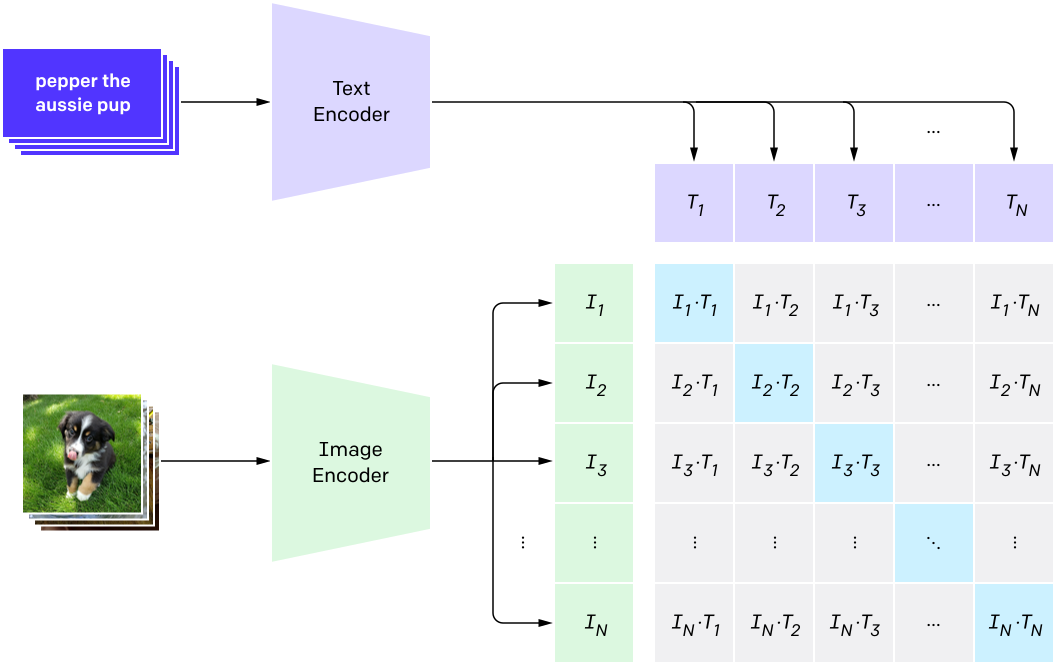
\includegraphics[width=0.7\linewidth]{../../figures/02-04-text-support-img/contrastive-pre-training}
    \caption{Visualization of contrastive objective \parencite{openai2021clipblog}}
  \end{figure}

  Drawback: Not as flexible as predictive objective, no image captioning
\end{frame}

\subsection{Zero shooting and foundation models} %------------------------
\begin{frame}{Concepts: Zero shooting and foundation models}
  \begin{itemize}
    \item Zero shooting
    \begin{itemize}
      \item Paradigm from NLP research
      \item Definition: Apply pre-trained model to new, unseen datasets
      \item No deceivement through overfitting
    \end{itemize}
    \item Foundation model: Model can be reused, e.g., CLIP is used inside DALL$\cdot$E 2 \parencite{ramesh2022hierarchical} to embed images
  \end{itemize}

  \begin{figure}[ht]
    \begin{minipage}{0.67\textwidth}
      \centering
      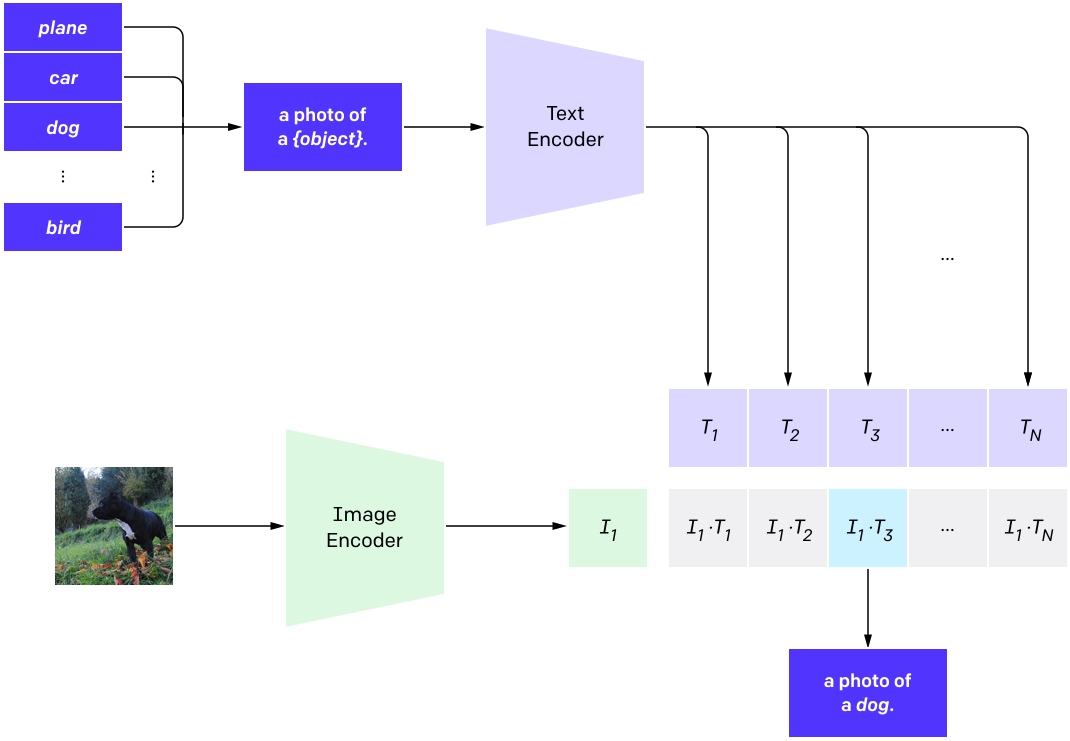
\includegraphics[width=0.9\linewidth]{../../figures/02-04-text-support-img/zero-shooting}
    \end{minipage}
    \begin{minipage}[c]{0.3\textwidth}
      \caption{Visualization of zero-shot application \parencite{radford2021learning}}
    \end{minipage}
  \end{figure}
\end{frame}

\subsection{Connecting image representations to language}
\begin{frame}{Concepts: Connecting image representations to language}
  \begin{itemize}
    \item Learned representations are directly connected to natural language
    \item Direct specification of visual concepts possible through prompt engineering, e.g., \enquote{picture of ...}, \enquote{macro of ...} or \enquote{drawing of ...}
  \end{itemize}
\end{frame}

\section{Architectures} %-------------------------------------------------

\subsection{CLIP}
\begin{frame}{CLIP}
  
\end{frame}

% Also the chosen transformer using architectures allow for large sample sizes, aggressive parallelization

\subsection{ALIGN}
\begin{frame}{ALIGN}
  
\end{frame}

\subsection{Florence}
\begin{frame}{Florence}
  
\end{frame}


\section{Performance comparison} %----------------------------------------
\begin{frame}{Performance comparison}
  \begin{table}[ht]
    \centering
    \resizebox{\textwidth}{!}{
    \begin{tabular}{l|rrrr|rrrr}
      \hline
      & \multicolumn{4}{c}{Flickr30K (1K test set)}
      & \multicolumn{4}{|c}{MSCOCO (5K test set)}  \\
      & \multicolumn{2}{c}{Image$\rightarrow$Text}
      & \multicolumn{2}{c}{Text$\rightarrow$Image}
      & \multicolumn{2}{|c}{Image$\rightarrow$Text}
      & \multicolumn{2}{c}{Text$\rightarrow$Image} \\
               & R@1           & R@5           & R@1           & R@5           & R@1           & R@5           & R@1           & R@5           \\
      \hline
      CLIP     & 88.0          & 98.7          & 68.7          & 90.6          & 58.4          & 81.5          & 37.8          & 62.4          \\
      ALIGN    & 88.6          & 98.7          & 75.7          & \textbf{93.8} & 58.6          & 83.0          & 45.6          & 69.8          \\
      Florence & \textbf{90.9} & \textbf{99.1} & \textbf{76.7} & 93.6          & \textbf{64.7} & \textbf{85.9} & \textbf{47.2} & \textbf{71.4} \\
      \hline
    \end{tabular}
    }
    \caption{Zero-shot retrieval}
  \end{table}
\end{frame}

\section{Resources} %-----------------------------------------------------
\begin{frame}{Resources}
  \begin{itemize}
    \item rclip
  \end{itemize}
\end{frame}

\section{Sources} %-------------------------------------------------------
\begin{frame}[allowframebreaks]{Sources}
  \printbibliography[heading=bibnumbered, title = Bibliography]
\end{frame}

\end{document} %----------------------------------------------------------
